\documentclass[11pt]{article}
\setlength{\textwidth6.5in} \setlength{\textheight9.3in}
\setlength{\oddsidemargin0in} \setlength{\topmargin-0.7in}
\setlength{\unitlength}{1cm}

\def\squarebox#1{\hbox to #1{\hfill\vbox to #1{\vfill}}}
\newcommand{\qedbox}{\vbox{\hrule\hbox{\vrule\squarebox{.667em}\vrule}\hrule}}
\newcommand{\qed}{\nopagebreak\mbox{}\hfill\qedbox\bigskip}
\def\solution{\textbf{Solution: }}

\usepackage{times}
\usepackage[T1]{fontenc}
\usepackage{graphics}
\usepackage{graphicx}
%\usepackage[english]{babel}
\usepackage{subfig}
\usepackage{amssymb}
\usepackage{amsmath}
\usepackage{amsfonts}
\usepackage{enumerate}
\usepackage{hyperref}
\usepackage{eurosym}
\usepackage{wrapfig}
\usepackage{float}
\usepackage{multirow}
\usepackage[most]{tcolorbox}
\usepackage{enumitem}

\newcommand{\ra}{\rightarrow}
\newcommand{\ua}{\uparrow}
\newcommand{\prob}[1]{P\left(#1\right)}
\newcommand{\imp}{\Rightarrow}
\newcommand{\re}{\mathbb{R}}
\newcommand{\Exp}[1]{\mathbb{E}\left[#1\right]} %Expectation

% KEEP THIS FOR FINAL VERSION, COMMENT FOR DRAFTING STAGE
%\newcommand{\comment}[1]{}


\begin{document}

%-----------------This is the header/topics portion--------------------
\noindent \rule{\textwidth}{.5mm} \noindent \makebox[1.5in][l]{\bf
  CMS/CS/EE/IDS 144} \hfill \makebox[1.5in][r]{\bf Gurus: Tia \& Han}

  \vspace{0.25cm}

\noindent \centerline{\bf {\Large HW 5: Centrality \& Games}}

\vspace{0.25cm}

\noindent \makebox[1.5in][l]{Assigned: 02/13/2026} \hfill
\makebox[1.5in][r]{Due: 02/19/2026 by 11:59 PM PT} \noindent
\rule{\textwidth}{.5mm}

%-----------------This is the header/topics portion--------------------

\noindent \textit{Collaboration is allowed for all problems and at the top of your homework sheet, please list all the people with whom you discussed. Crediting help from other classmates will not take away any credit from you. The details of the collaboration policy for this course are available in the Resources tab on Piazza.}\\

\noindent \textit{You must turn in your homework electronically via Gradescope. \textbf{Be sure to submit your homework as a single file.}}\\

\noindent \textit{Start early and come to office hours with your questions! We also encourage you to post your questions on Piazza, as well as answer the questions asked by others on Piazza.}

\noindent \rule{6in}{0.4pt}
\section*{Coding + Data Analysis [70 points]}
\rule{6in}{0.4pt}

%\setcounter{section}{-1}
\section{Discovering Clusters [40 points]}

\noindent In class, you have seen the power of clustering on many real world applications. The choice of clustering algorithm depends on both the structures of graphs and the metrics used for clustering, among other things. In this problem, you will evaluate various clustering algorithms on a couple of different types of graphs: symmetric stochastic block model (SSBM), as seen in \textbf{Homework 2}, and the "circle graph", to get a sense for the differences between algorithms. \\


\noindent \textbf{Your task:}

\begin{enumerate}[label=(\alph*)]

\item \textbf{[20 points]}
Generate a SSBM network with $n=30, k=3, A=0.7$ and $B=0.1$. Run the spectral clustering and $k$-means clustering algorithms over the network, for appropriate value(s) of $k,$ and visualize the clusters obtained from each algorithm. You may find Python libraries such as \texttt{sklearn.cluster.KMeans} and \texttt{sklearn.cluster.SpectralClustering} useful for this question. 

\begin{tcolorbox}[colback=gray!10, colframe=gray!50, title=Reminder]
The \textit{stochastic block model (SBM)} is a random graph model with planted clusters. %It generalizes the {\em Erd\H{o}s--R\'{e}nyi} model and is widely employed as a canonical model to study clustering and community detection, which are central problems in machine learning and data mining. 
The model $SBM(n, p, W)$ defines an $n$-vertex random graph with labeled vertices for positive integers $n$, $k$, a probability vector $p$ of dimension $k$, and a symmetric matrix $W$ of dimension $k \times k$ with entries $W_{i,j} \in [0, 1]$. Each vertex is assigned a community label in $\{1,..., k\}$ independently under the community prior $p$, and pairs of vertices with community labels $i$ and $j$ connect independently with probability $W_{i,j}$. The SBM is called \emph{symmetric} if $p$ is uniform and if $W$ takes the same value $A$ on the diagonal and the same value $B$ outside the diagonal. We then represent the symmetric SBM as $SSBM(n, k, A, B)$.
\end{tcolorbox}

 

Turn in a visualization of the results of your algorithms and a discussion of any differences you notice between the two algorithms. You may base this explanation on the visualization or some specific clustering metrics of your choice.  Also, discuss how well the clusters were recovered by these algorithms by comparing them to the actual clusters that were used to form the SSBM instance you generated.

\item \textbf{[20 points]} Generate an instance of the "circle graph", as seen below in Figure~\ref{fig:circle_graph}, with number of nodes $n = 500,$ and noise $\sigma = 0.01,$ using the \texttt{sklearn.datasets.make\_circles} function; half of the $n$ nodes will end up in the inner circle, and the other half in the outer circle. Run the spectral clustering and $k$-means clustering algorithms over the network, for appropriate value(s) of $k,$ and visualize the clusters obtained from each algorithm. Discuss any differences you notice between the two algorithms, and why any differences might occur. You will again find the aforementioned Python libraries useful for this problem.

\begin{figure}[H]
    \centering
    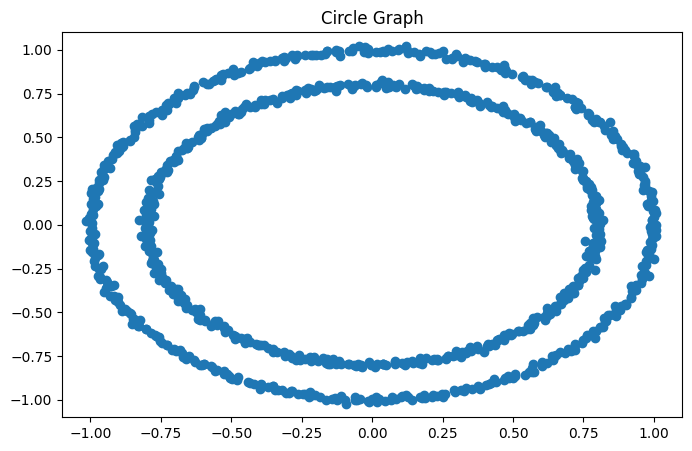
\includegraphics[width=0.75\linewidth]{figs/circle_graph.png}
    \caption{The Circle Graph with $n = 500, \sigma = 0.01$}
  \label{fig:circle_graph}
\end{figure}

 \end{enumerate}

\begin{tcolorbox}[colback=gray!10, colframe=gray!50, title=Note 1]
    The two clustering algorithms differ in that spectral clustering conventionally operates on a graph $G = (V, E)$ represented using an adjacency matrix (which is how the SSBM graph is represented), whereas $k$-means conventionally operates on a graph whose nodes are points in a vector space (which is how the circle graph is represented: a set of $(x,y)$ coordinate pairs). Therefore, in order to run spectral clustering on the circle graph, in addition to passing in the matrix of data points, you will need to pass in an "affinity" function, which essentially defines a metric by which the algorithm can build an adjacency graph from the points in the vector space; we suggest the \texttt{nearest\_neighbors} affinity function, which creates an adjacency matrix with edges between nodes that are close to each other in the vector space. When running $k$-means on the SSBM graph, you can simply pass in the adjacency matrix as is, or transform it as you see fit; regardless of which one you choose, as part of your discussion, talk about how the $k$-means algorithm is interpreting the data points you pass in to generate its clustering. Running $k$-means on the circle graph and running spectral clustering on the SSBM graph should follow naturally from the conventional definitions of the two algorithms.
\end{tcolorbox}

\begin{tcolorbox}[colback=gray!10, colframe=gray!50, title=Note 2]
For those of you interested in using a language/library besides Python/sklearn, the circle graph is created by first generating a vector of equally spaced points $\{r_1, \ldots, r_{n/2}\}$ in the interval $[0, 2\pi),$ then generates $(x, y)$ coordinate pairs according to $x_i^{\text{outer}} = (\cos(r_i), \sin(r_i))$ for the outer circle and $x_i^{\text{inner}} = f \cdot (\cos(r_i), \sin(r_i))$ for the inner circle, where $0 \leq f < 1$ (the make\_circles function uses $f = 0.8$ by default.) Then, a Gaussian error term $\epsilon_i \sim \mathcal{N}(0, \sigma^2)$ is added to the $x$ coordinate of each of the $n$ points, to give the final dataset.
\end{tcolorbox}

\section{Braess's Paradox Simulation [30 points]}

\noindent In game theory and traffic assignment, \textit{Braess's Paradox} is the counter-intuitive observation that adding road capacity to a network can sometimes \textit{increase} the overall travel time for everyone. This happens because individual drivers act selfishly to minimize their own travel time, reaching a Nash Equilibrium that is not necessarily the social optimum. The new road might offer a shortcut that looks attractive to individuals, but when everyone tries to use it, the resulting congestion slows the whole system down. In this problem, you will simulate this phenomenon to see how selfish routing decisions lead to suboptimal outcomes.

\begin{figure}[h]
    \centering
    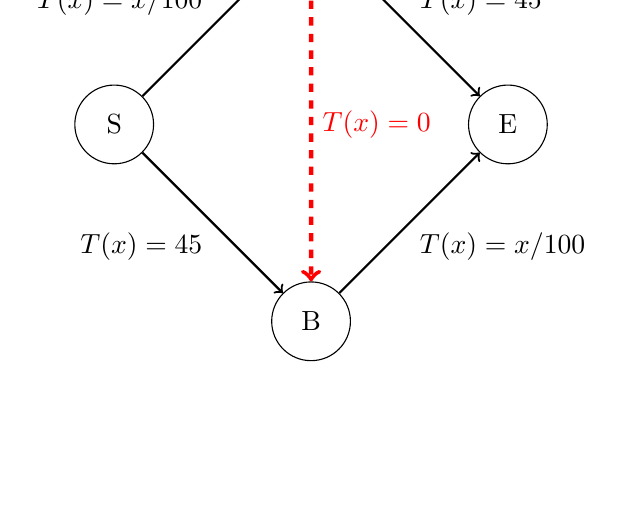
\begin{tikzpicture}[scale=1.25, auto, swap]
        % Nodes
        \node[draw, circle, minimum size=1cm] (S) at (0,2) {S};
        \node[draw, circle, minimum size=1cm] (A) at (2,4) {A};
        \node[draw, circle, minimum size=1cm] (B) at (2,0) {B};
        \node[draw, circle, minimum size=1cm] (E) at (4,2) {E};

        % Edges
        \draw[->, thick] (S) -- node[above left] {$T(x) = x/100$} (A);
        \draw[->, thick] (S) -- node[below left] {$T(x) = 45$} (B);
        \draw[->, thick] (A) -- node[above right] {$T(x) = 45$} (E);
        \draw[->, thick] (B) -- node[below right] {$T(x) = x/100$} (E);
        
        % The Paradox Edge (Dashed)
        \draw[->, dashed, ultra thick, red] (A) -- node[right] {$T(x) = 0$} (B);
    \end{tikzpicture}
    \caption{The Traffic Network. Solid lines are the initial state; the dashed line is the upgrade.}
\end{figure}

\noindent \textbf{Your task:} Simulate 4000 drivers traveling from $S$ to $E$.

\begin{enumerate}[label=(\alph*)]
\item \textbf{[10 points]} Initialize all drivers on the top ($S \to A \to E$) path. Iteratively move 1\% of the drivers currently on the slowest path to the fastest path; do this 1,000 times. Assume drivers act greedily, are rational, and make their decisions in each iteration simultaneously. Generate a plot showing average travel time for each path and overall v. iteration number. Report the final number of drivers on each path and the average travel time. Does this appear to be an equilibrium?

\item \textbf{[10 points]} Add the zero-cost edge $A \to B$, creating a third path ($S \to A \to B \to E$). Continuing from the final distribution of drivers between the top and bottom paths from the previous part, now allow drivers to switch to any of the three paths. Generate a plot showing average travel time for each path and overall v. iteration number. Report the new average travel time and the final number of drivers on each path. Does this appear to be an equilibrium? Did the average travel time increase or decrease? 


\item \textbf{[10 points]} Explain intuitively why rational drivers flocked to the new path despite it worsening the global outcome. Why don't they switch back?
\end{enumerate}


\newpage
\noindent \rule{6in}{0.4pt}
\section*{Theory [30 Points]}
\rule{6in}{0.4pt}


\section{Eavesdropping Centrality [15 points]}

For this problem, you'll study a new notion of centrality. The idea behind the measure is that the "importance" of a node in a communication network is, in some sense, tied to the desire of an eavesdropper to monitor network communication by "bugging" that node. If the node would be really important for an eavesdropper to bug then the node is "central" in some sense.\\

\noindent Concretely, consider the following setting.

\begin{itemize}
\item \textbf{Communication Process:} Between time 0 and time 1, each vertex sends a (different) message to each of its neighbors independently at a uniformly random time, i.e., for each edge $(i,j)$, $T_{ij}$ is the time $i$ sends a message to $j$ and is distributed between $[0, 1)$ independently of all other edges.

\item \textbf{Eavesdropping Process:} At any time between time 0 and time 1 the eavesdropper can "bug" any set of nodes in the network and intercept the incoming messages. But, the probability the eavesdropper is caught by node $i$ at the end of the round is $t_i^{\beta}$ where $t_i$ is the total time spent at node $i$ during the round and $\beta$ is a parameter. The events of being caught at node $i$ and node $j$ are not independent.
\end{itemize}

\noindent The policy of the eavesdropper is $t = (t_1, \ldots, t_n)$, which specifies how much time each node is monitored and the goal of the eavesdropper is to maximize the expected number of messages intercepted during the round while making sure that the probability of being caught is smaller than $\gamma$, where $\gamma \in (0, 1)$.\\

\noindent Intuitively, the importance of a node is proportional to the amount of time it is bugged by a strategic eavesdropper.

\begin{enumerate}[label=(\alph*)]
\item \textbf{[5 points]} Given policy $t = (t_1, \ldots, t_n)$, show that the expected number of intercepted messages is $\sum_{i=1}^n t_i d_i$ where $d_i$ is the degree of node $i$.

\item \textbf{[5 points]} Prove that if $\sum_{i=1}^n t_i^{\beta} \leq \gamma$, then the probability of being caught is at most $\gamma$. This means that such a $t = (t_1, \ldots, t_n)$ is a valid policy.

\item \textbf{[5 points]} Given \textbf{parts (a)} and \textbf{(b)}, we obtain an optimization problem that can be solved to determine the vector of eavesdropper centrality, $t^*$:
\begin{equation}
t^* = \arg \max \sum_{i=1}^n t_i d_i \text{ subject to } \sum_{i=1}^n t_i^{\beta} \leq \gamma.
\end{equation}

Note that this problem uses a bound on the probability of being caught. We'll ignore that fact for this homework, but please convince yourself why that's okay! Our goal in this problem is to connect the idea of eavesdropping centrality to the notions of centrality in the previous problem.

To that end, consider two specific cases: $\beta = 1$ and $\beta = 2$. For each of these cases, solve the optimization problem and interpret the resulting $t^*$ as a centrality measure, connecting it to the centrality measures in the previous problem. \textit{(Hint: The Cauchy-Schwarz inequality may be useful.)}
\end{enumerate}

\section{Game Theory Warm Up [10 points]}

This question is designed to put in use the concepts you learned in the \textbf{game theory refresher lecture}. Remember that for each element in the table, $(x, y)$ represents a payoff of $x$ for Player 1 and $y$ for Player 2.

\begin{center}
\begin{tabular}{cc|c|c|c|c|}
\multicolumn{2}{c}{} & \multicolumn{4}{c}{Player 2} \\
\multicolumn{2}{c}{} & $a$ & $b$ & $c$ & $d$ \\
\cline{3-6}
\multirow{4}{*}{Player 1} & $w$ & $(3, 2)$ & $(4, 1)$ & $(4, 0)$ & $(2, 1)$ \\
\cline{3-6}
& $x$ & $(2, 4)$ & $(5, 3)$ & $(5, 5)$ & $(0, 3)$ \\
\cline{3-6}
& $y$ & $(2, 1)$ & $(3, 3)$ & $(3, 0)$ & $(0, 6)$ \\
\cline{3-6}
& $z$ & $(1, 3)$ & $(4, 6)$ & $(5, 4)$ & $(3, 1)$ \\
\cline{3-6}
\end{tabular}
\end{center}

\noindent Consider the two-player normal form game given above.

\begin{enumerate}[label=(\alph*)]
\item \textbf{[5 points]} Which actions survive the iterated elimination of dominated actions? Explain your claim.

\item \textbf{[5 points]} Find all Nash Equilibria \textit{(Hint: you should find 2 pure and 2 mixed)}.
\end{enumerate}

\section{Routing Games with Tolls [5 points]}

In our discussion of routing games in class, we talked about using tolls to induce independent selfish players to behave in a manner that is optimal for the system. To this end, we discussed the principle of \emph{marginal cost pricing}. In this exercise, you'll prove that marginal cost pricing really works.\\

\noindent Consider the model of routing games described in class. Assume that each user $i$ has traffic $r_i = 1.$ We add a `toll' to the original link cost functions $c_e(\cdot),$ setting the new cost function to be

$$c^*_e(x) = c_e(x) + (x-1)\left(c_e(x) - c_e(x-1)\right)$$

\noindent Notice that the `toll' on link $e$ captures the net latency that each player using the link adds to the other players using it.\\


\noindent \textbf{Your Task: } Prove that any optimal strategy for our original game is a Nash equilibrium for this new game (with link cost functions $c^*_e(\cdot)$). Recall that the objective function in the original game is $\sum_{i \in N}\sum_{e \in E_i}c_e(f_e)=\sum_{e \in E} f_e c_e(f_e)$ where $f_e$ is the flow on $e$, $N$ is the set of players and $E_i$ contains the edges on the path selected by player $i$. \textit{(Hint: Think about constructing a new potential function with the new cost.)}

\end{document}

